% Adapted from: http://web.mit.edu/rsi/www/pdfs/beamer-tutorial.tex

\documentclass[pdf]{beamer}
\mode<all>{\usetheme{Warsaw} \useoutertheme{split}}
\mode<handout>{\usecolortheme{seagull}}
%\usepackage{rsislidepacks}
\usepackage{amsfonts}
\usepackage{amsmath}
\usepackage{amssymb}
\usepackage{amsthm}
\usepackage{graphicx}
\usepackage{url}
%
\usepackage{colortbl}
\usepackage{epstopdf}
\usepackage{eurosym}
\usenavigationsymbolstemplate{}
\usepackage{gensymb}
\newcommand\Fontvi{\fontsize{8}{7.2}\selectfont}
\newcommand\Fontpi{\fontsize{6}{4}\selectfont}

\usepackage{siunitx}
\usepackage{verbatim}
\usepackage{booktabs}
\usepackage{tfrupee}  
\pdfmapfile{=tfrupee.map}
\newcommand{\specialcell}[2][l]{%
	\begin{tabular}[#1]{@{}l@{}}#2\end{tabular}}
\usepackage{multirow}
\setbeamerfont{section in toc}{size=\small}
\setbeamerfont{subsection in toc}{size=\tiny}

\addtobeamertemplate{navigation symbols}{}{%
	\usebeamerfont{footline}%
	\usebeamercolor[fg]{footline}%
	\hspace{1em}%
	\insertframenumber/\inserttotalframenumber
}

%Free and Open Source libraries of Python for all geospatial I/O

\title[\tiny \hspace{145pt} ICPAC]{Python for Climate Scientist}
\author[Python for Climate Scientist]{Nishadh K. A. \newline \newline  }

\begin{document}
	
\AtBeginSection[]{
	\begin{frame}{Table of Contents}
		\tableofcontents[currentsection]
	\end{frame}
}

\begin{frame}
	\thispagestyle{empty}
	\titlepage
\end{frame}
\addtocounter{framenumber}{-1}

\begin{frame}{Table of Contents}
	\tableofcontents
\end{frame}
%\begin{frame}{Outline}
%\begin{itemize}
%\item Python background
%\item Setting up Python
%\item Python Libraries for Climate Science
%\item Data exploration and visulazation 
%\item Functions and Command lines programs 	
%\item Demo prgrams 
%\end{itemize}
%
%
%\end{frame}


\section[Python background]{Python background}

\begin{frame}{Python's holy grail!}
	
	\only<1>{\centering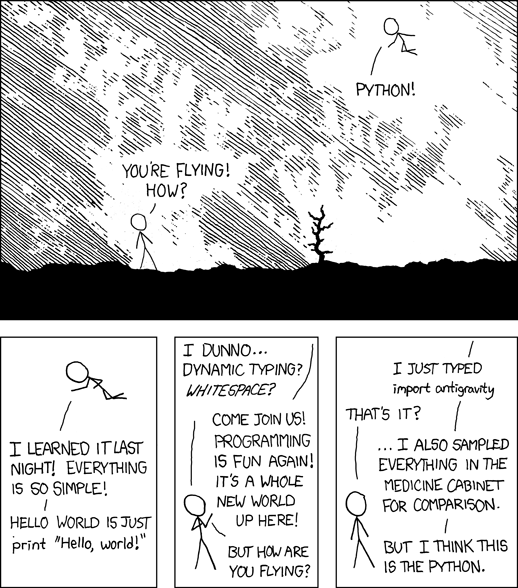
\includegraphics[scale=0.33]{python.png}} 
	
\end{frame}

\begin{frame}{Advantages of Python}
	%\Fontvi
	\begin{beamerboxesrounded}{}
		"I have used a combination of Perl, Fortran, NCL, Matlab, R and others for routine research, but found out this general- purpose language, Python, can handle almost all in an efficient way from requesting data from remote online sites to statistics, and graphics."
		by a scientist
	\end{beamerboxesrounded}
\end{frame}



\begin{frame}{Python - Characteristics}
	%\Fontvi
	\begin{beamerboxesrounded}{}
		\begin{itemize}
			\item Easy to read and learn
			\item High-level language
			\item General-purpose language
			\item Interpreted language
			\item Extensive libraries
			\item Large userbase 
		\end{itemize}
	\end{beamerboxesrounded}
\end{frame}



\begin{frame}{Free and open-source software (FOSS)}
	%\Fontvi
	\begin{beamerboxesrounded}{}
		\begin{itemize}
			\item The freedom to run
			\item The freedom to study 
			\item The freedom to redistribute
			\item The freedom to distribute copies
		\end{itemize}
	\end{beamerboxesrounded}
    	\begin{beamerboxesrounded}{}
    	\begin{itemize}
    		\item Free Software- Ethical imperative, Liberty
    		\item Open Source- software development practice
    	\end{itemize}
    \end{beamerboxesrounded}

\end{frame}


\section[Setting up Python]{Setting up Python}

\begin{frame}{Endeavor of setting up Python- it is all included!}
	
	\only<1>{\centering\includegraphics[scale=0.23]{flayer_httyc.png}} 
	
	\begin{itemize}
		\item Anaconda!
		\item Docker
- "The life boat"
		\item Version Control System
- "Time travelling"
		\item Jupyter Notebooks
- "Galileo Galilei's Notebook"
		\item Markdown - "Better formatted notes"
	\end{itemize}

\end{frame}

\subsection[Anaconda!]{Anaconda!}

\begin{frame}{Anaconda- Python distribution}
	%\Fontvi
	\begin{beamerboxesrounded}{}
		\begin{itemize}
			\item Open source package manager
			\item Virtual environment 
			\item Extensively helped in improve user base
			\item Greater coverage on Data science and machine learning 
		\end{itemize}
	\end{beamerboxesrounded}
\end{frame}


\subsection[The life boat-Docker]{The life boat-Docker}

\begin{frame}{Life boat}
	%\Fontvi
	\begin{beamerboxesrounded}{}
		\begin{itemize}
			\item Virtualization
			\item OS as folders
			\item Docker 
			\item Organized as layers 
		\end{itemize}
	\end{beamerboxesrounded}
\end{frame}



\subsection[Time travelling-The git]{Time travelling-The git}
\begin{frame}{Time travelling}
	%\Fontvi
	\begin{beamerboxesrounded}{}
		\begin{itemize}
			\item Version control system
			\item Used in Software development, collaborative document writing
			\item Parallel to science 
		\end{itemize}
	\end{beamerboxesrounded}
\end{frame}

%\subsection[Galileo Galilei's Notebook]{Galileo Galilei's Notebook}
\subsection[Jupyter notebook]{Jupyter notebook}

\begin{frame}{Galileo Galilei's  Starry Messenger}
	%\Fontvi
	\begin{beamerboxesrounded}{}
		\begin{itemize}
			\item Data in publication
			\item Scientific reproducibility
			\item more reading https://www.theatlantic.com/science/archive/2018/04/the-scientific-paper-is-obsolete/556676/ 
		\end{itemize}
	\end{beamerboxesrounded}
\end{frame}

\begin{frame}{Literal programming}
	%\Fontvi
	\begin{beamerboxesrounded}{}
		\begin{itemize}
			\item By Donald Knuth, Stanford University
			\item Readable text with Code section
			\item Well suited for Demonstration, research, and teaching 
			\item A major shift in writing code denoted with thought porcess and background information related to the code 
			\item Jupyter notebooks are for Literal programming
		\end{itemize}
	\end{beamerboxesrounded}
\end{frame}


\begin{frame}{What are Jupyter notebooks}
	%\Fontvi
	\begin{beamerboxesrounded}{}
		\begin{itemize}
			\item A command shell for interactive computing
			\item A browser-based notebook with support for code, text, mathematical expressions, inline plots and other media.
			\item For  introspection, rich media, shell syntax, tab completion, and history.
			\item Language agnostic 
			\item Enhances interactive data visualization and use of GUI toolkits.
			\item Easily shareable 
			\item enables parallel computing 
		\end{itemize}
	\end{beamerboxesrounded}
\end{frame}

\begin{frame}{Markdown language}
	%\Fontvi
	\begin{beamerboxesrounded}{}
		\begin{itemize}
			\item Text component of notebooks
			\item Lightweight markup language
			\item Defacto writing language in web
			\item Simple syntax
		\end{itemize}
	\end{beamerboxesrounded}
\end{frame}

















%\begin{frame}
%	\only<1-2>{show\_me\_first}
%	\only<2>{show\_me\_second}
%\end{frame}
\section[Libraries for Climate Science]{Libraries for Climate Science}
%\section[Component 2]{Component 2: Measure a line}
\begin{frame}{Libraries for Climate Science}
	
	\only<1>{\centering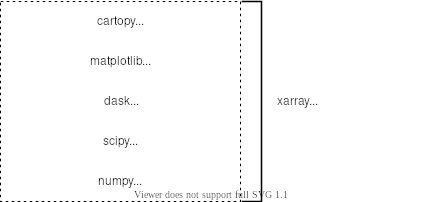
\includegraphics[scale=0.85]{01-pyaos-stack.png}} 
	
\end{frame}

\begin{frame}{Libraries for GIS}
	
	\only<1>{\centering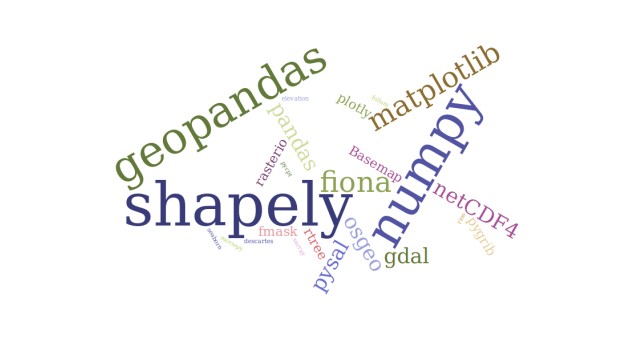
\includegraphics[scale=0.53]{gis_libs.png}} 
	
\end{frame}

\begin{frame}{Libraries gives kind of Neo's vision on Climate Data}
	
	\only<1>{\centering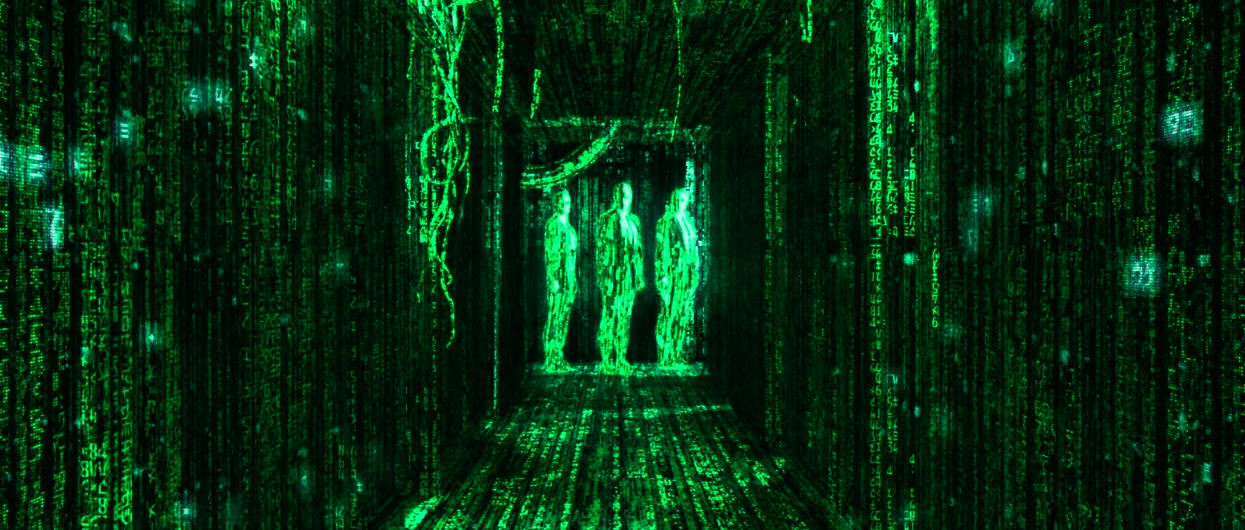
\includegraphics[scale=0.33]{neo_vision.png}} 
	
\end{frame}


\begin{frame}{Python libraries for raster operations}
	%\Fontvi
	\begin{beamerboxesrounded}{}
		\begin{itemize}
			\item rasterio gives tools to read geotiff
			\item Convert the satellite imagery into simple numpy array
			\item Several algorithm to clean and detect features in imagery
		\end{itemize}
	\end{beamerboxesrounded}
\end{frame}


\begin{frame}{Python libraries for vector operations}
	\begin{beamerboxesrounded}{}
		\begin{itemize}
			\item Geopandas to read the shape file
			\item Shapely to perform various vector operation
			\item Rtree index for spatial indexing of large data sources
		\end{itemize}
	\end{beamerboxesrounded}
\end{frame}

\section[Data exploration and visualization ]{Data exploration and visualization}

\begin{frame}{Data exploration and visualization}
	\begin{beamerboxesrounded}{Contents based on }
		\begin{itemize}
			\item https://carpentries-lab.github.io/python-aos-lesson/
		\end{itemize}
	\end{beamerboxesrounded}
	\begin{beamerboxesrounded}{To work on}
		\begin{itemize}
			\item Import the xarray library and use the functions it contains
			\item Convert precipitation units to mm/day
			\item Calculate and plot the precipitation climatology
			\item Use the cmocean library to find colormaps designed for ocean science
		\end{itemize}
	\end{beamerboxesrounded}
\end{frame}


\section[Functions and Command lines programs]{Functions and Command lines programs}

\begin{frame}{Functions and Command lines programs}
	\begin{beamerboxesrounded}{To work on}
		\begin{itemize}
			\item Define a function that takes parameters
			\item Use docstrings to document functions
			\item Break our existing plotting code into a series of small, single-purpose functions
			\item Use the argparse library to manage command-line arguments in a program
			\item Structure Python scripts according to a simple template
		\end{itemize}
	\end{beamerboxesrounded}
\end{frame}

\section[Demo Programs]{Demo Programs}

\begin{frame}{Demo Programs}
	\begin{beamerboxesrounded}{To work on}
		\begin{itemize}
			\item Read GFS data and plot maps
			\item Wind animation from GFS data
		\end{itemize}
	\end{beamerboxesrounded}
\end{frame}


\section[]{}

\begin{frame}{}
	\Large
	
	Thank you
	
\end{frame}   
\end{document}



%total slides=50
%GenralIntro=5
%StudyArea=2
%Chapter1=10
%Chapter2=10
%Chapter3=10
%Chapter4=10
%ConcuFutrDir=3
%GenralIntro
%1-ParticulatePollution
%2-IssuesInterventionMeasures
%3-DataIntensiveApproach
%4-studyObjectives
%5-ThesisOrganization
%StudyArea
%1-CurrentStatus
%2-InterventionMeasures
%Chapter1
%Introcution=1
%Methodology=2
%Results=6
%Conculsion=1
%Chapter2
%Introcution=1
%Methodology=2
%Results=6
%Conculsion=1
%Chapter3
%Introcution=1
%Methodology=2
%Results=6
%Conculsion=1
%Chapter4
%Introcution=1
%Methodology=2
%Results=6
%Conculsion=1
%ConcuFutrDir=3
